% !TeX root = ../main.tex

%\section{Killer Whale Case Study}

\subsection{Data Collection and Preprocessing}

To apply this methodology to real-world data, the CarHHMM was used to analyze dive data from a killer whale off the coast of British Columbia, Canada. The data was collected on September 2, 2019 from 12:49 pm to 6:06 pm and consists of depth and acceleration in three orthogonal directions. Observations were collected at a rate of 50 hertz. Tagging the killer whale caused anomalous behavior before 1:20 pm and after 6:00 pm, so observations in this time range were ignored. In addition, the tagging technology dropped data between 2:25pm and 2:37pm as well as between 4:07 and 5:07 pm, so any partially observed data within this time range were ignored as well. A killer whale ``dive" is considered to be any continuous chunk of data that occurs below 0.5 meters in depth and lasts for at least 10 seconds. Accelerometer and depth data were smoothed by taking a moving average with a window of 1/10th of a second. Data preprocessing was done in part with the \textit{divebomb} package in Python \citep{Nunes:2018}. After preprocessing the raw data, a total of 267 dives were observed. A plot of the raw data for all dives and a collection of five selected dives can be seen in figures \ref{fig:data} and \ref{fig:data_one_dive}, respectively.

\begin{figure}[ht]
	\centering
	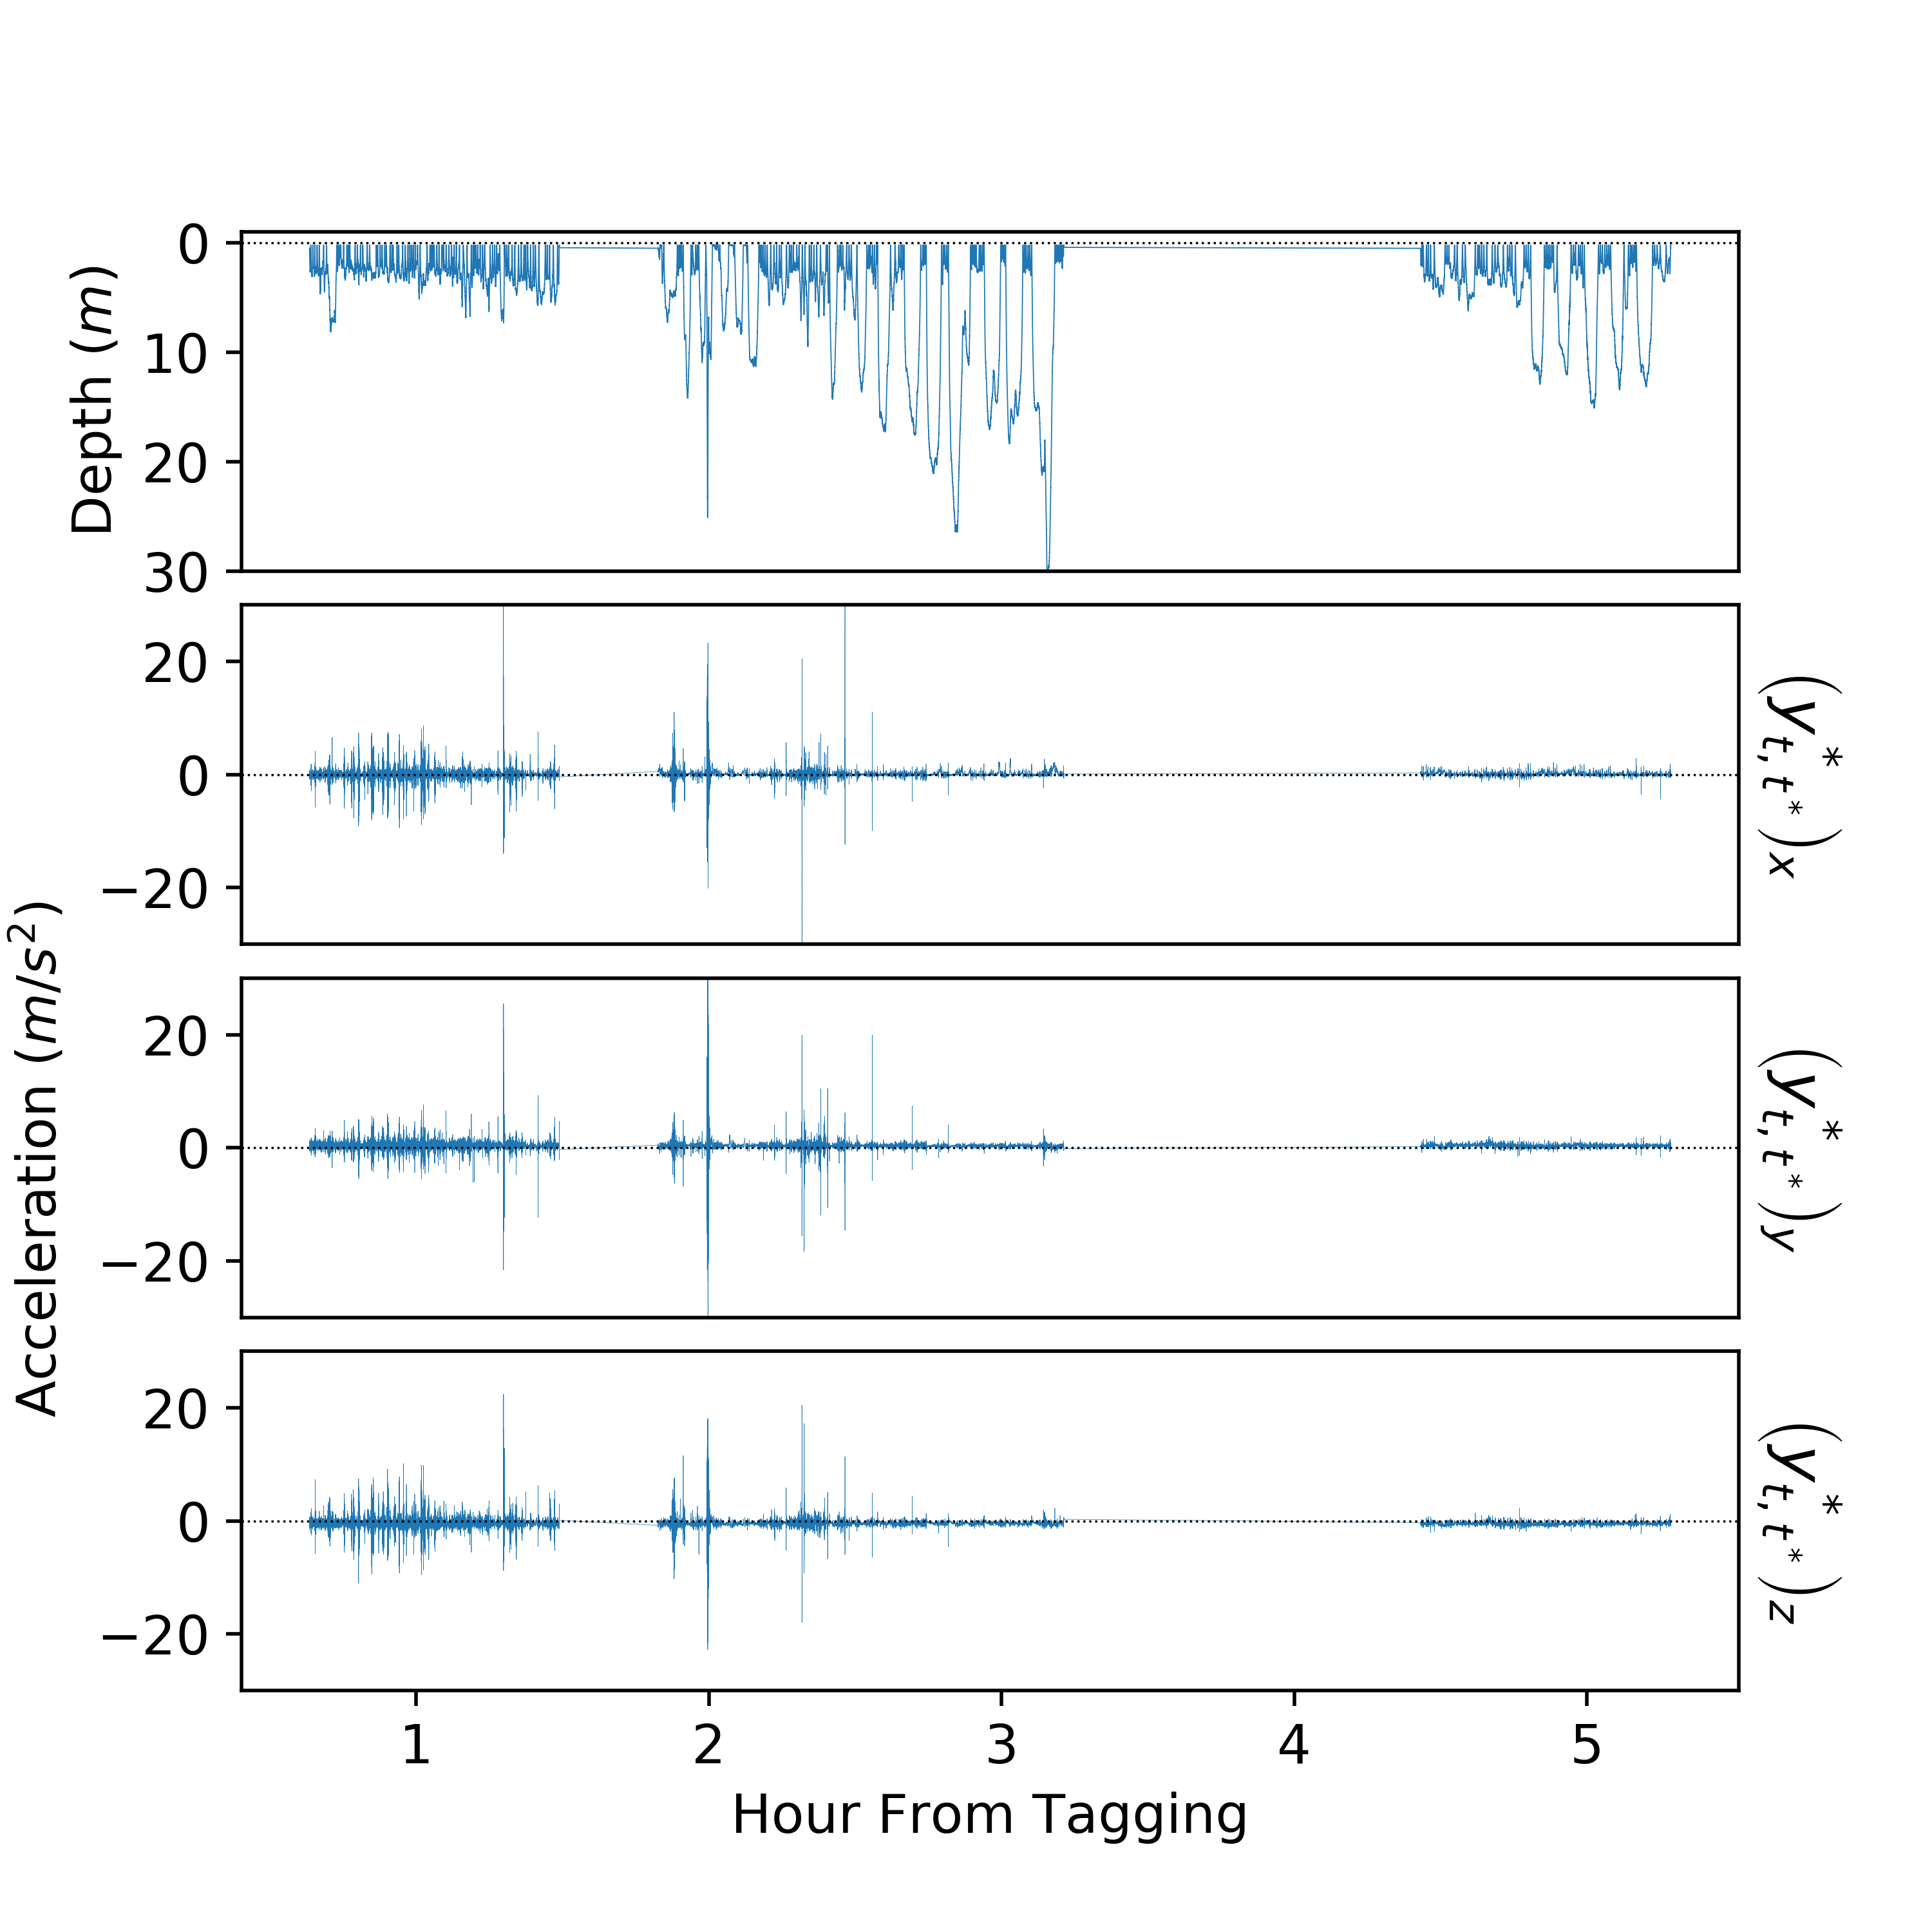
\includegraphics[width=5in]{../Plots/raw_data.png}
	\caption{Dive profile and Acceleration data of entire data set}
	\label{fig:data}
\end{figure}

\begin{figure}[ht]
	\centering
	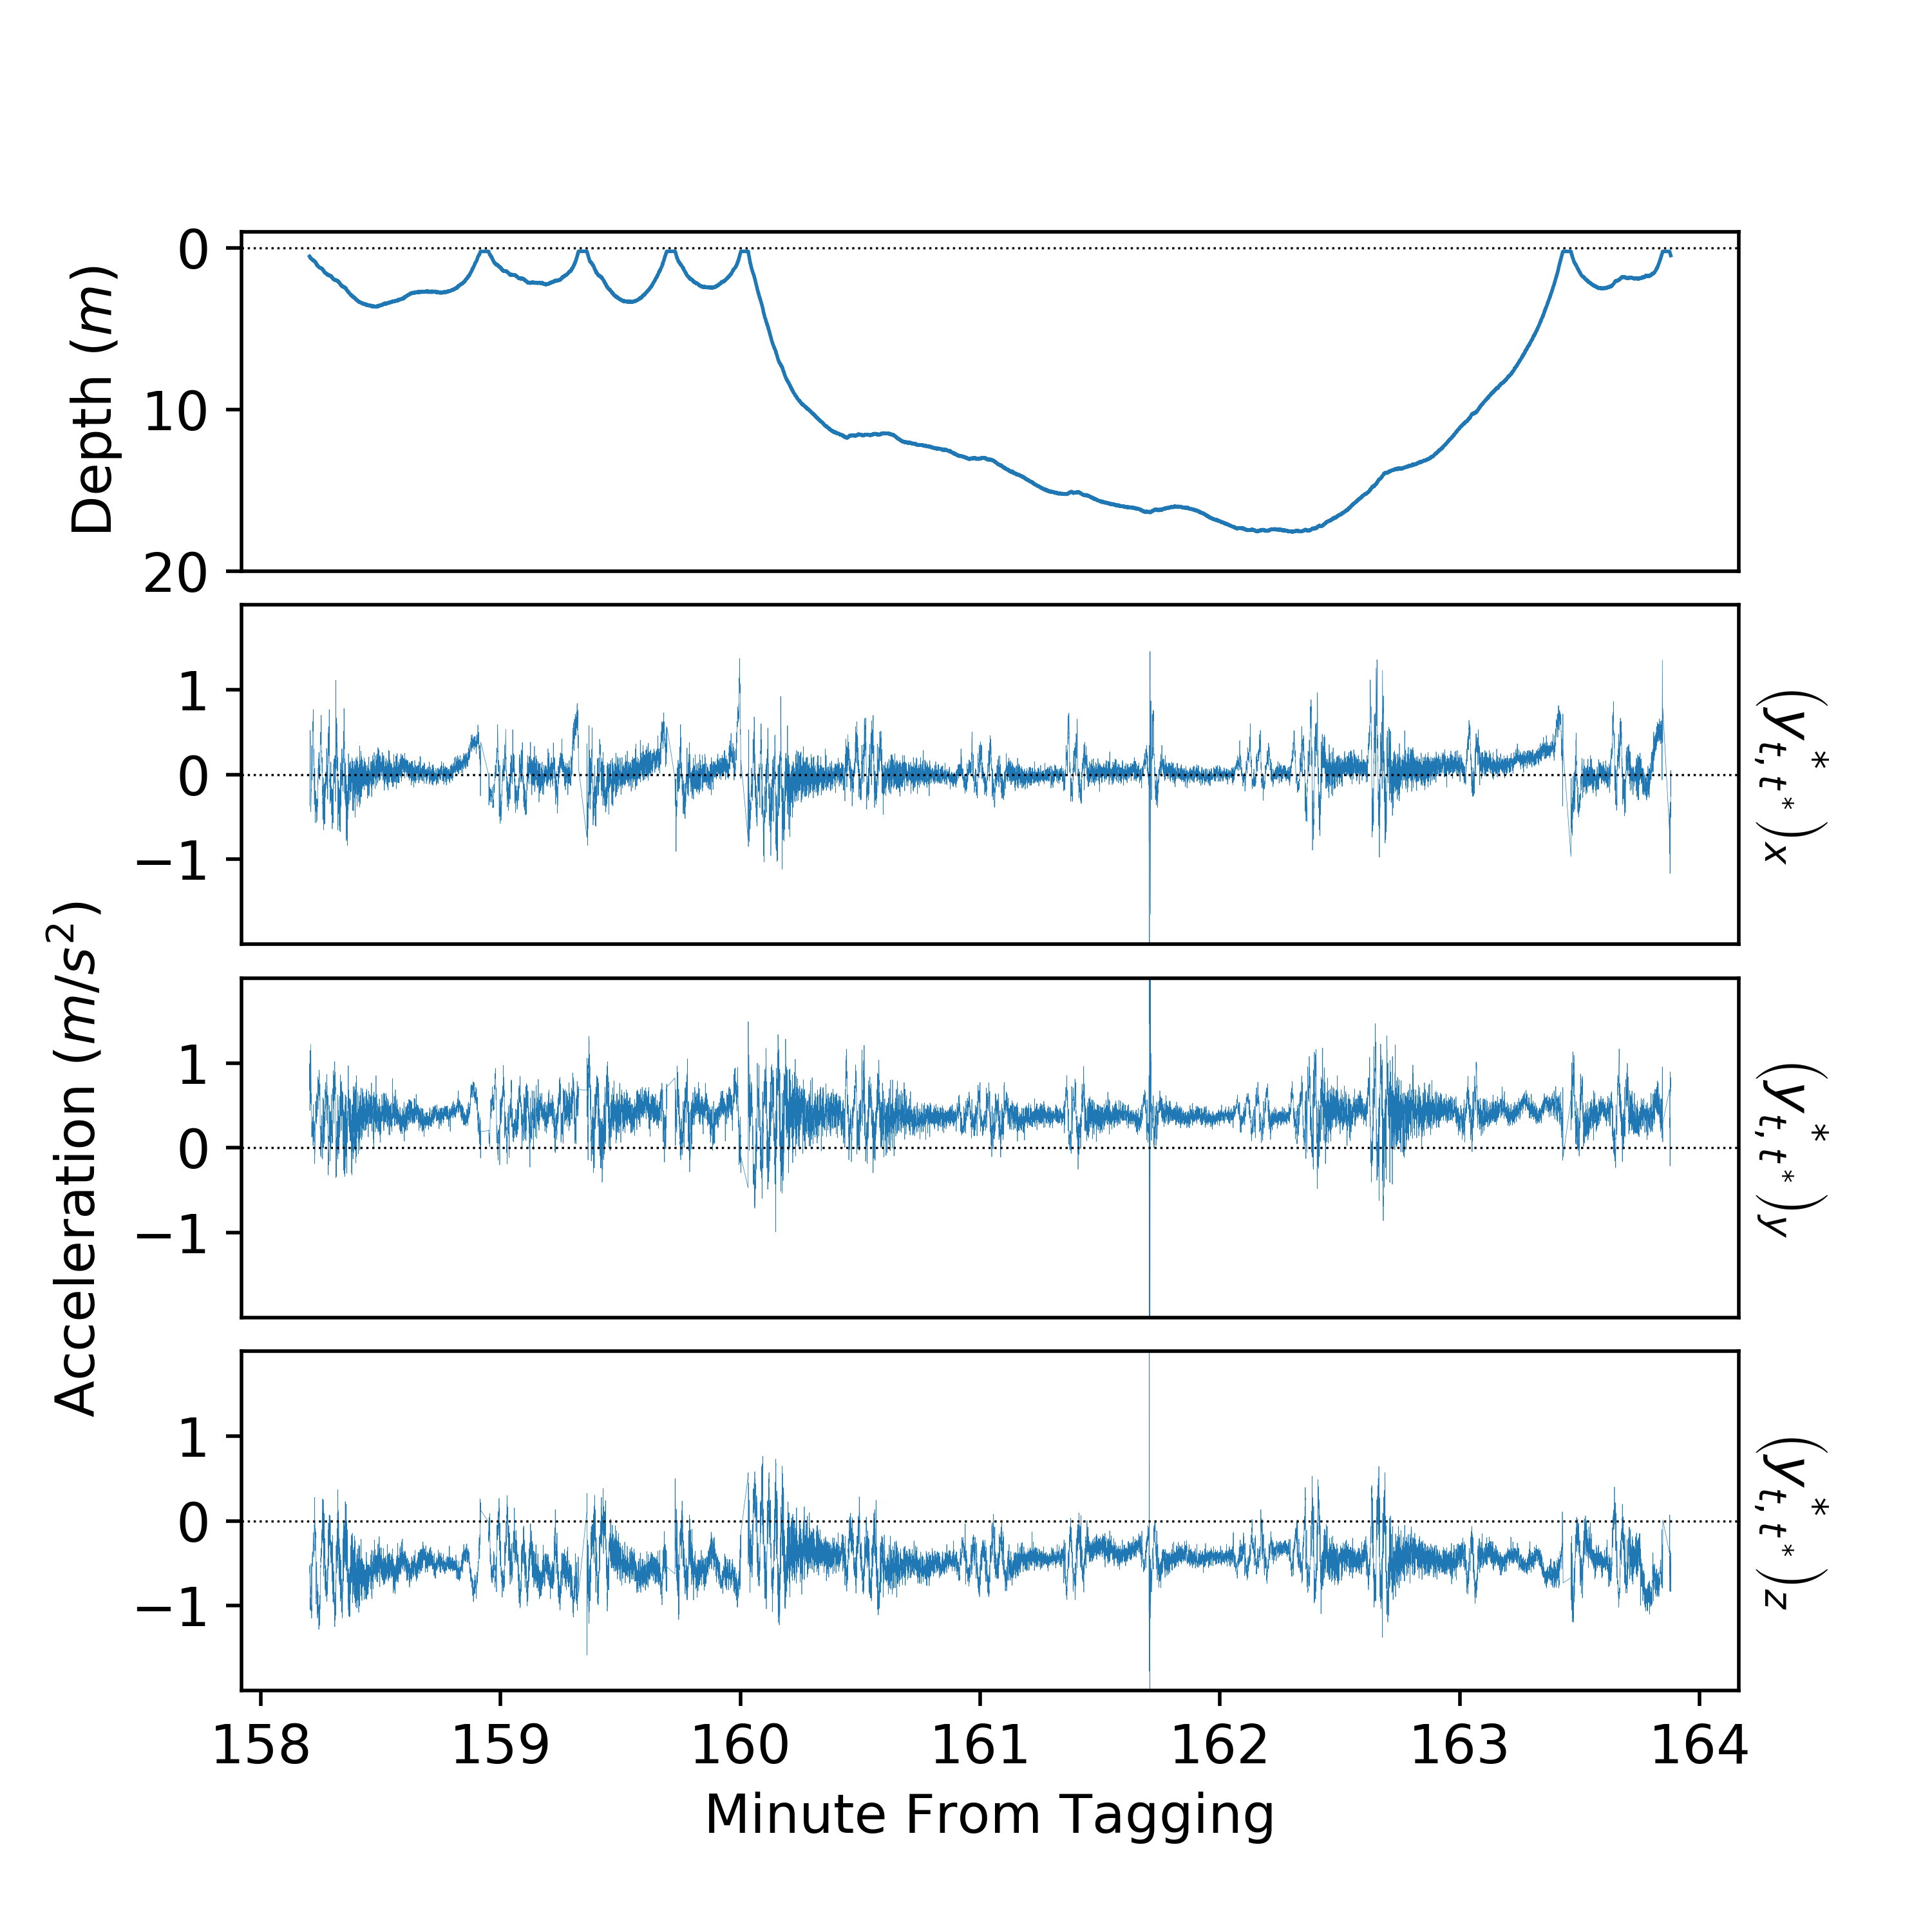
\includegraphics[width=5in]{../Plots/raw_data_5_dives.png}
	\caption{Dive profile and acceleration data for a collection of 5 dives of a killer whale.}
	\label{fig:data_one_dive}
\end{figure}

\subsection{Model Selection}

The collection of all dive durations were set to be the coarse-scale observations $Y$, and the acceleration data was used to determine the fine-scale observations $Y^*$. The acceleration exhibits sinusoidal behavior at several points in time which cannot be modeled using HMMs without some kind of signal processing (see fig \ref{fig:data_one_dive}). Therefore, the STFT was used to calculate both $Y^{*(1)}$ and $Y^{*(2)}$ as described in section \ref{subsec:STFT}. We set $\tilde{f} = 5$ hertz and $h = 2$ seconds, which reduced the dimension of each window from $50 s^{-1} * 2 s = 100$ to $2$.

To determine if the CarHHMM was appropriate for this data, a lag plot was made for both $Y^{*(1)}_{t,s^*}$ and $Y^{*(2)}_{t,s^*}$, as shown in figure (\ref{fig:lag}). The number of behavioral states is not clear from the lag plot, but it is clear that $Y^{*(1)}_{t,s^*}$ exhibits a large degree of auto-correlation, so the CarHMM was used for $Y^{*(1)}_{t,s^*}$. The auto-correlation parameter $\hat phi$ was set to be shared among all dimensions of $Y^{*(1)}_{t,s^*}$, but both the means and variances were allowed to be different. While $Y^{*(2)}_{t,s^*}$ also exhibits some auto-correlation, the relationship is less strong. In addition, the biological interpretation of auto-correlation within $Y^{*(2)}_{t,s^*}$ is more difficult than for $Y^{*(1)}_{t,s^*}$, so auto-correlation was not incorporated into the emission distribution of $Y^{*(2)}_{t,s^*}$.

\begin{figure}[ht]
	\centering
	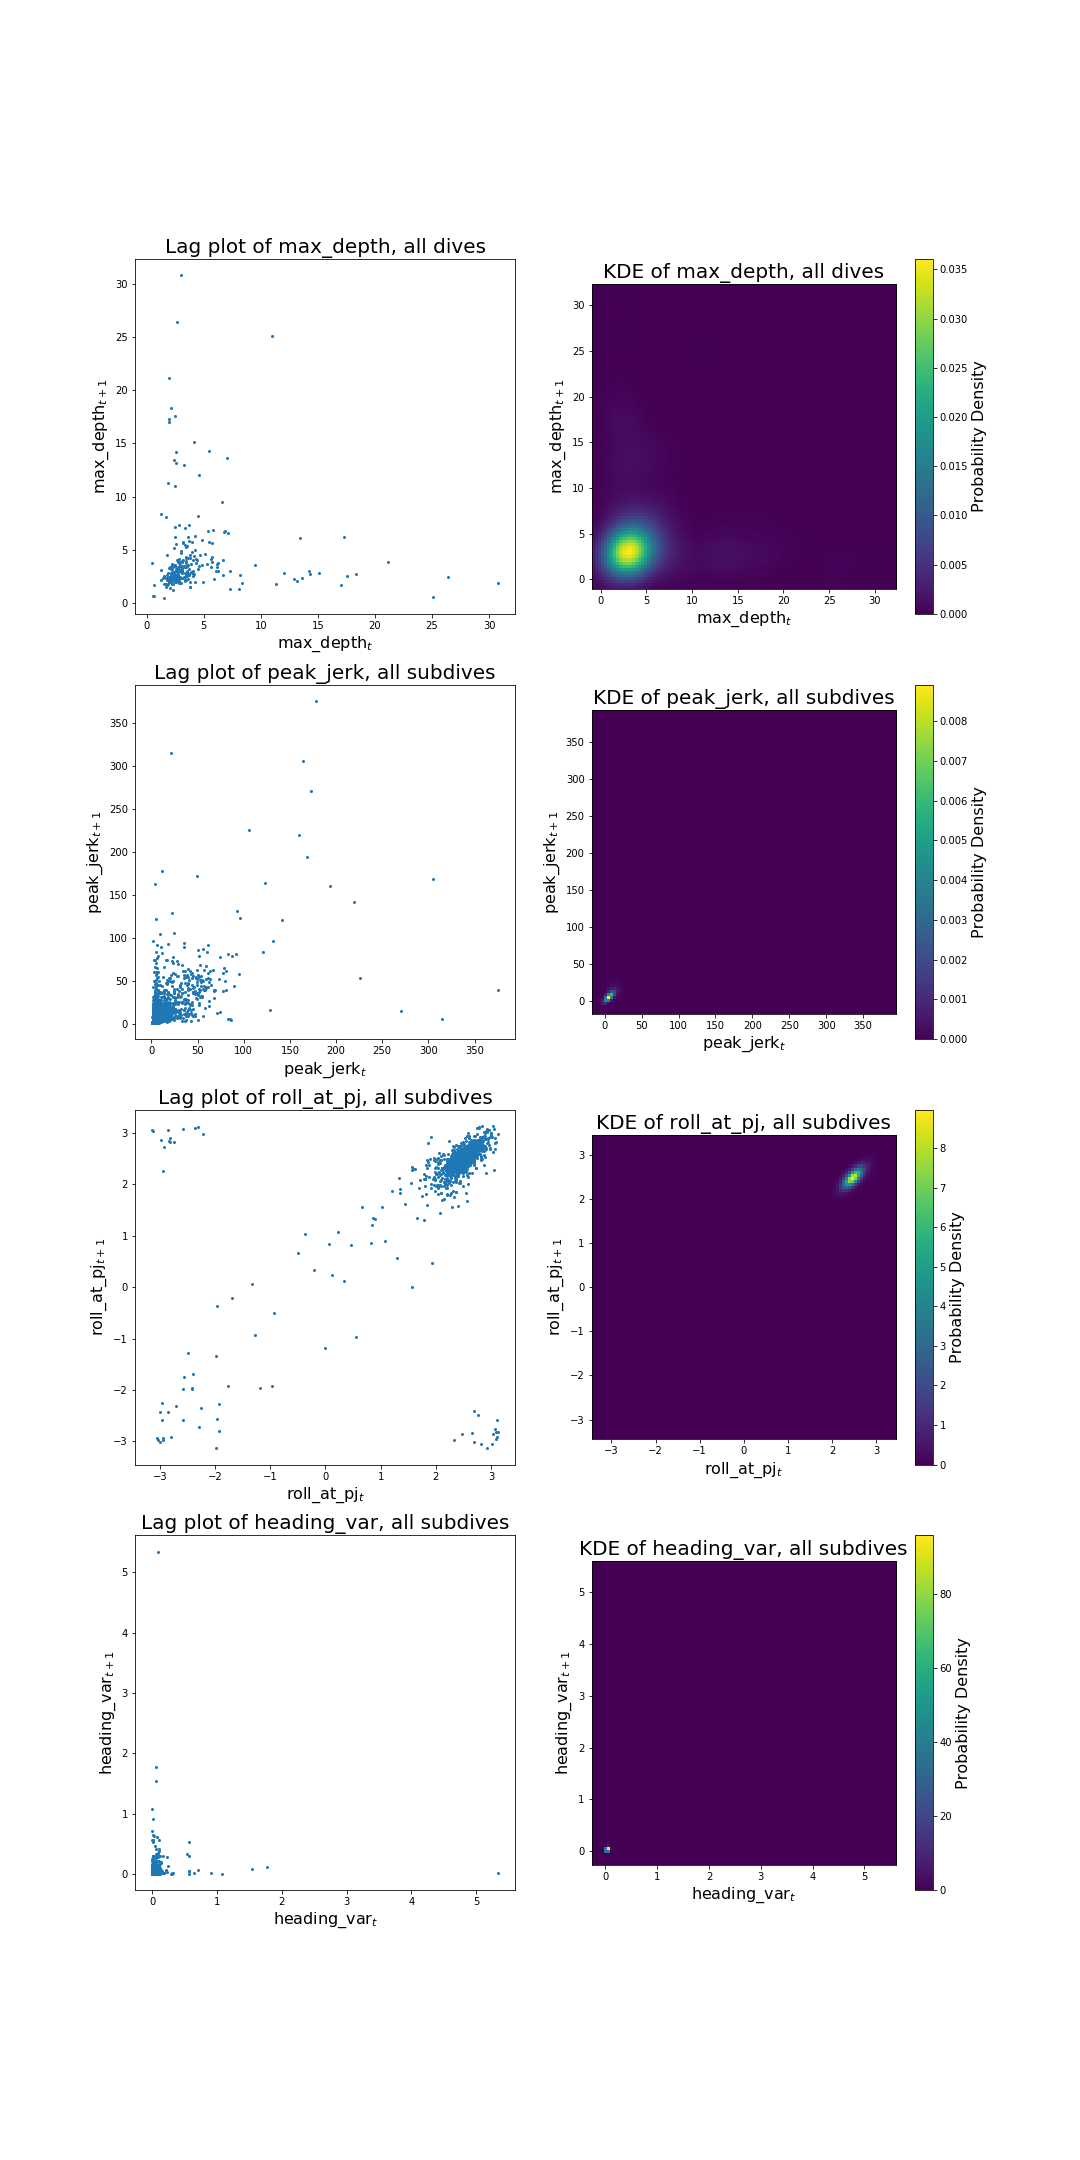
\includegraphics[height=7in]{../Plots/lagplot.png}
	\caption{Lag plot of all features (left) and the associated normal kernel density estimates (right)}
	\label{fig:lag}
\end{figure}

It is known that information criteria tends to overestimate the number of states in biological processes \citep{Pohle:2017}, so we instead selected $N = 2$ dive types and $N^* = 3$ sub-dive behaviours heuristically and admittedly somewhat arbitrarily. The absence of principled tool to select the number of hidden states is a common issue in statistical ecology. Therefore, it is important to use model validation techniques in lieu of information criteria. Section \ref{subsec:model_validation} describes our process of validating this model in particular.

\subsection{Results}

The parameters of the estimated emission distributions for each behavioral state are shown in (table \ref{table:emis_dists}). Each distribution is also plotted in (fig \ref{fig:coarse_emis}) and (fig \ref{fig:fine_emis}). Note that the auto-correlation within the acceleration sequence is not captured in (fig \ref{fig:fine_emis}), so it is important to refer to the estimated auto-correlation parameter $\hat \phi$ from (table \ref{table:emis_dists}) when considering the emission distributions shown in (fig \ref{fig:fine_emis}).
%
\begin{figure}[ht]
	\centering
	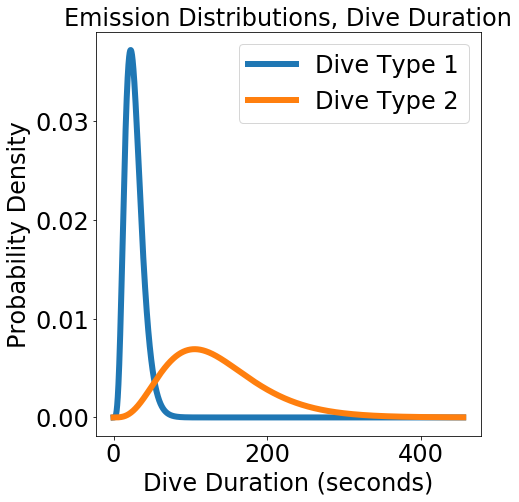
\includegraphics[height=4in]{../Plots/coarse-emissions.png}
	\caption{Estimated probability distributions for each coarse-scale observation in each dive type.}
	\label{fig:coarse_emis}
\end{figure}
%
\begin{figure}[ht]
	\centering
	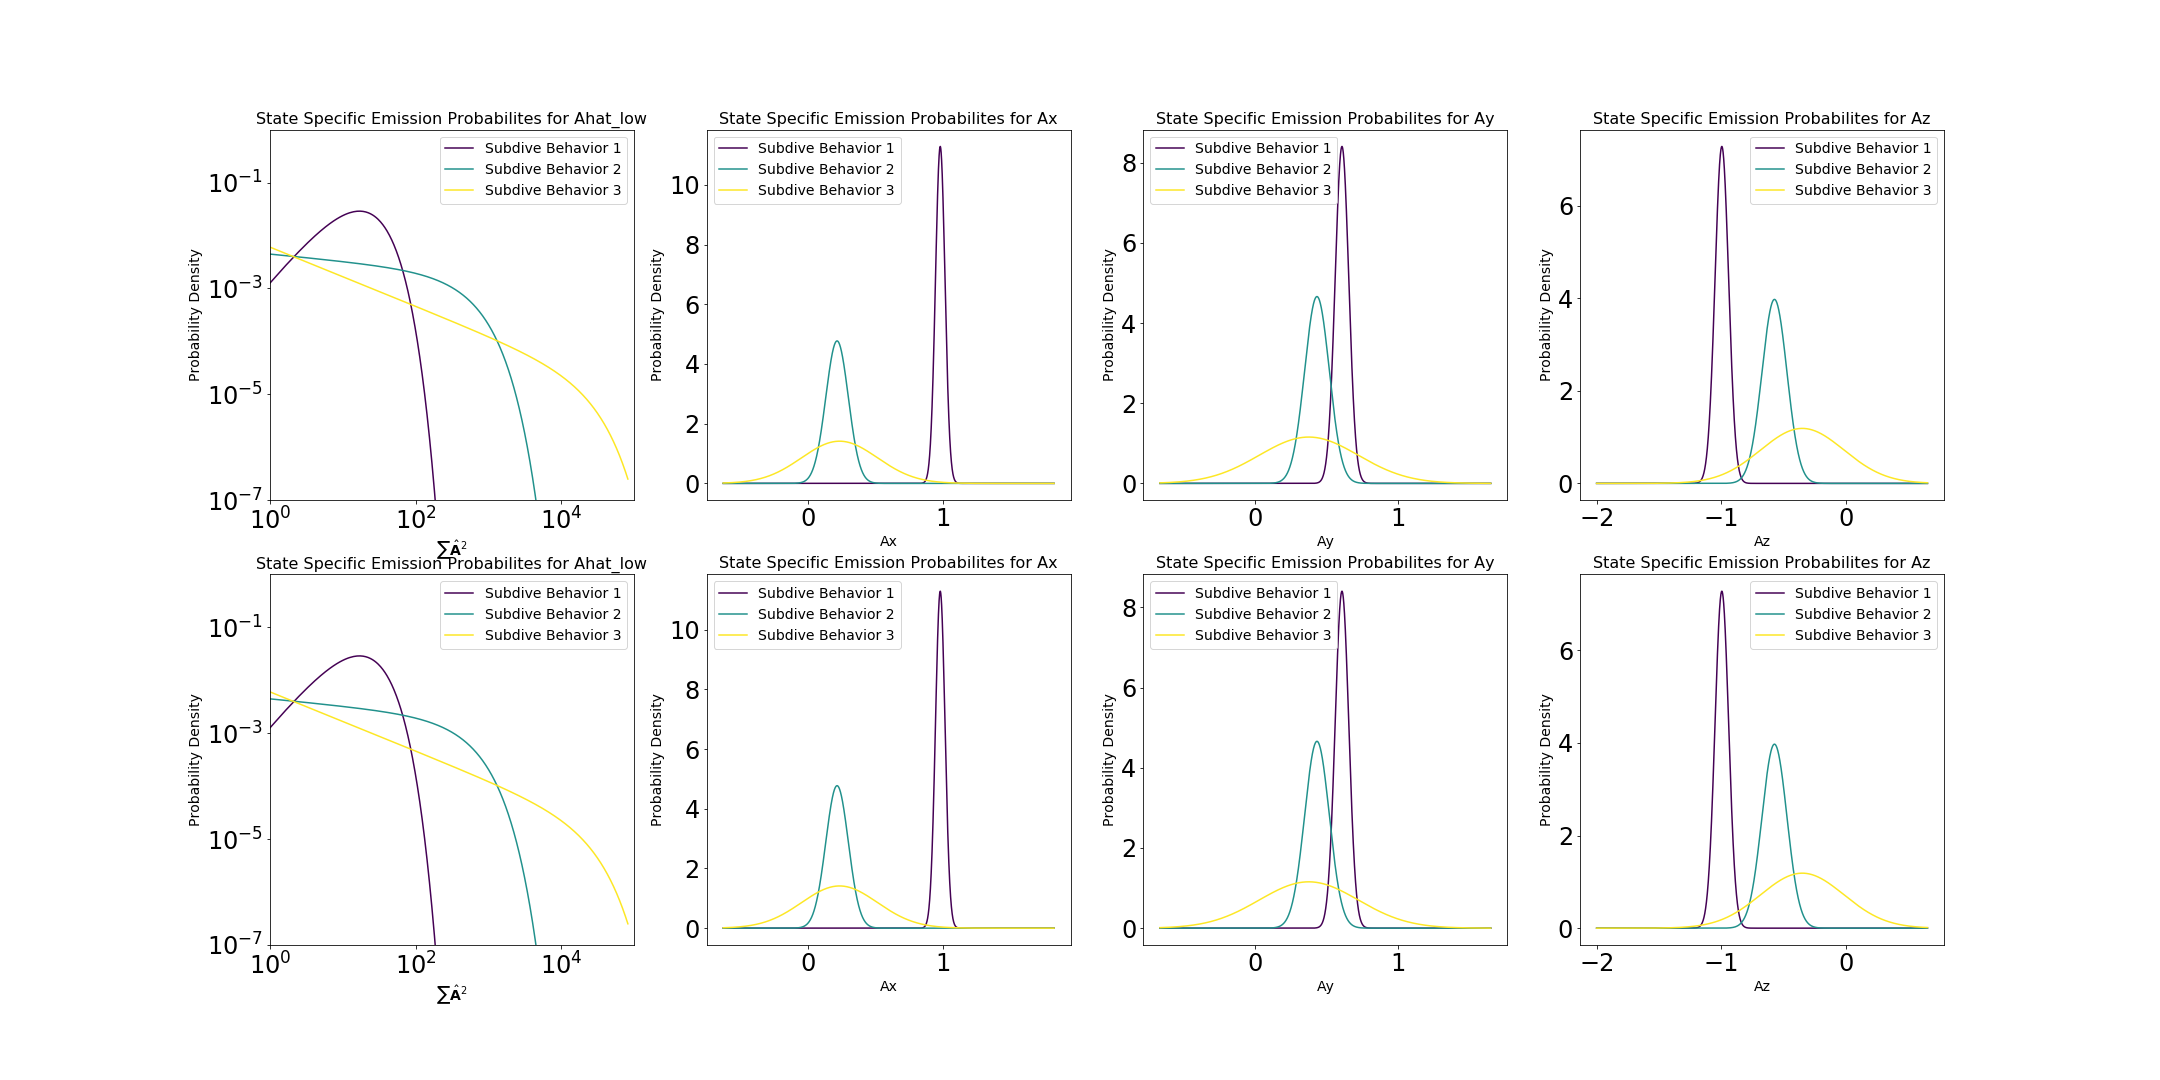
\includegraphics[height=2.5in]{../Plots/fine-emissions.png}
	\caption{Estimated probability distributions for each fine-scale observation in each behavioral state. Note that the distributions of acceleration does not take auto-correlation into account.}
	\label{fig:fine_emis}
\end{figure}
%
\begin{table}[ht]
    \centering
    \caption{Estimates and standard errors of emission parameters for killer whale data.}
    \scalebox{0.8}{
    \begin{tabular}{ccccc}
    \multirow{2}{*}{Feature}                 & \multirow{2}{*}{Dive / Sub-dive Type} & \multicolumn{3}{c}{Parameter Estimate}              \\
                                             &                                      & $\hat \mu$      & $\hat \sigma$   & $\hat \phi$     \\ \hline
    \multirow{2}{*}{Dive Duration (seconds)} & 1                                    & $27.23 \pm 0.63$ & $10.89 \pm 0.56$ & ---             \\
                                             & 2                                    & $127.96 \pm 11.50$ & $64.13 \pm 9.21$ & ---             \\ \hline
    \multirow{3}{*}{$Y^{*(1)}_x$}            & 1                                    & $0.98 \pm 0.07$ & $0.04 \pm 0.00$ & $0.99 \pm 0.00$ \\
                                             & 2                                    & $0.22 \pm 0.01$ & $0.08 \pm 0.00$ & $0.87 \pm 0.01$ \\
                                             & 3                                    & $0.23 \pm 0.03$ & $0.28 \pm 0.01$ & $0.62 \pm 0.03$ \\ \hline
    \multirow{3}{*}{$Y^{*(1)}_y$}            & 1                                    & $0.61 \pm 0.09$ & $0.05 \pm 0.00$ & $0.99 \pm 0.00$ \\
                                             & 2                                    & $0.43 \pm 0.01$ & $0.09 \pm 0.00$ & $0.87 \pm 0.01$ \\
                                             & 3                                    & $0.38 \pm 0.04$ & $0.35 \pm 0.01$ & $0.62 \pm 0.04$ \\ \hline
    \multirow{3}{*}{$Y^{*(1)}_z$}            & 1                                    & $-1.00 \pm 0.11$ & $0.05 \pm 0.00$ & $0.99 \pm 0.00$ \\
                                             & 2                                    & $-0.57 \pm 0.01$ & $0.10 \pm 0.00$ & $0.87 \pm 0.01$ \\
                                             & 3                                    & $-0.35 \pm 0.04$ & $0.34 \pm 0.01$ & $0.62 \pm 0.04$ \\ \hline
    \multirow{3}{*}{$Y^{*(2)}$}              & 1                                    & $27.16 \pm 0.32$ & $16.67 \pm 0.32$ & ---             \\
                                             & 2                                    & $406.98 \pm 4.42$ & $438.09 \pm 5.49$ & ---             \\
                                             & 3                                    & $9688.54 \pm 221.95$ & $14584.02 \pm 358.40$ & ---             \\ \hline
    \end{tabular}
    }
    \label{table:emis_dists}
\end{table}
%
While the ecological meaning of the modeled behavioral states is tenuous, we hypothesize the following interpretations. For the coarse scale, dive type 1 corresponds to shorter, shallower dives which serve a variety of purposes, including to rest before performing a dive of type 2, which corresponds to a deeper, more sustained dive. For the fine scale, behavioral state 1 corresponds to gliding and less overall activity of the whale compared to the other behavioral states. The mean of $Y^{*(2)}$ in this state is at least an order of magnitude smaller than sub-dive behavior 2, the variance of $Y^{*(1)}$ is smaller than sub-dive behavior 2, and the auto-correlation of $Y^{*(1)}$ is higher than every other behavioral state. This indicates a relatively constant acceleration and therefore low levels of activity. Sub-dive state 3 corresponds to vigorous swimming activity, as the mean of $Y^{*(2)}$ and variance of $Y^{*(1)}$ are much higher than every other state. The auto-correlation of $Y^{*(1)}$ is also much lower in this state, implying more variation in acceleration every 2 seconds. Sub-dive state 2 corresponds to a medium amount of activity, as almost every parameter estimate is between the other two behavioral states.

The estimated probability transition matrices and associated stationary distributions are shown below:
%
$$\hat \Gamma = \begin{pmatrix} 
0.849 & 0.151 \\
0.907 & 0.093
\end{pmatrix}$$
$$\hat \delta = \begin{pmatrix} 0.857 & 0.143 \end{pmatrix}$$
%
$$\hat \Gamma^{*(1)} = \begin{pmatrix} 
0.724 & 0.276 & 0.000 \\
0.057 & 0.887 & 0.056 \\
0.000 & 0.247 & 0.753
\end{pmatrix} \qquad 
\hat \Gamma^{*(2)} = \begin{pmatrix} 
0.871 & 0.129 & 0.000 \\
0.135 & 0.829 & 0.036 \\
0.000 & 0.246 & 0.754
\end{pmatrix}$$
$$\hat \delta^{*(1)} = \begin{pmatrix} 0.143 & 0.698 & 0.159 \end{pmatrix} \qquad
\hat \delta^{*(2)} = \begin{pmatrix} 0.476 & 0.456 & 0.067 \end{pmatrix}$$
%
About 86\% of observed dives are short- the whale usually rests for many dives in a row before performing a deep dive. Interestingly, the probability transition matrix $\hat \Gamma$ shows that the current dive does not effect the dive type of the following dive much. In addition, the fine-scale probability transition matrices imply that the killer whale is much more likely to be in a less active sub-dive state when performing deep dives than when performing shallow dives- 14\% of shallow dives are spent in sub-dive state 1 while 48\% of deep dives are spent in sub-dive state 1. Using less active sub-dive states when diving deep could be an energy reduction strategy for these long periods of holding breath.

The decoded dive behavior within 5 selected dives is shown in (fig \ref{fig:labeled_dives}). In addition, the probability of each dive type and sub-dive state is shown in (fig \ref{fig:coarse_probs}) and (fig \ref{fig:fine_probs}), respectively.

\begin{figure}[ht]
	\centering
	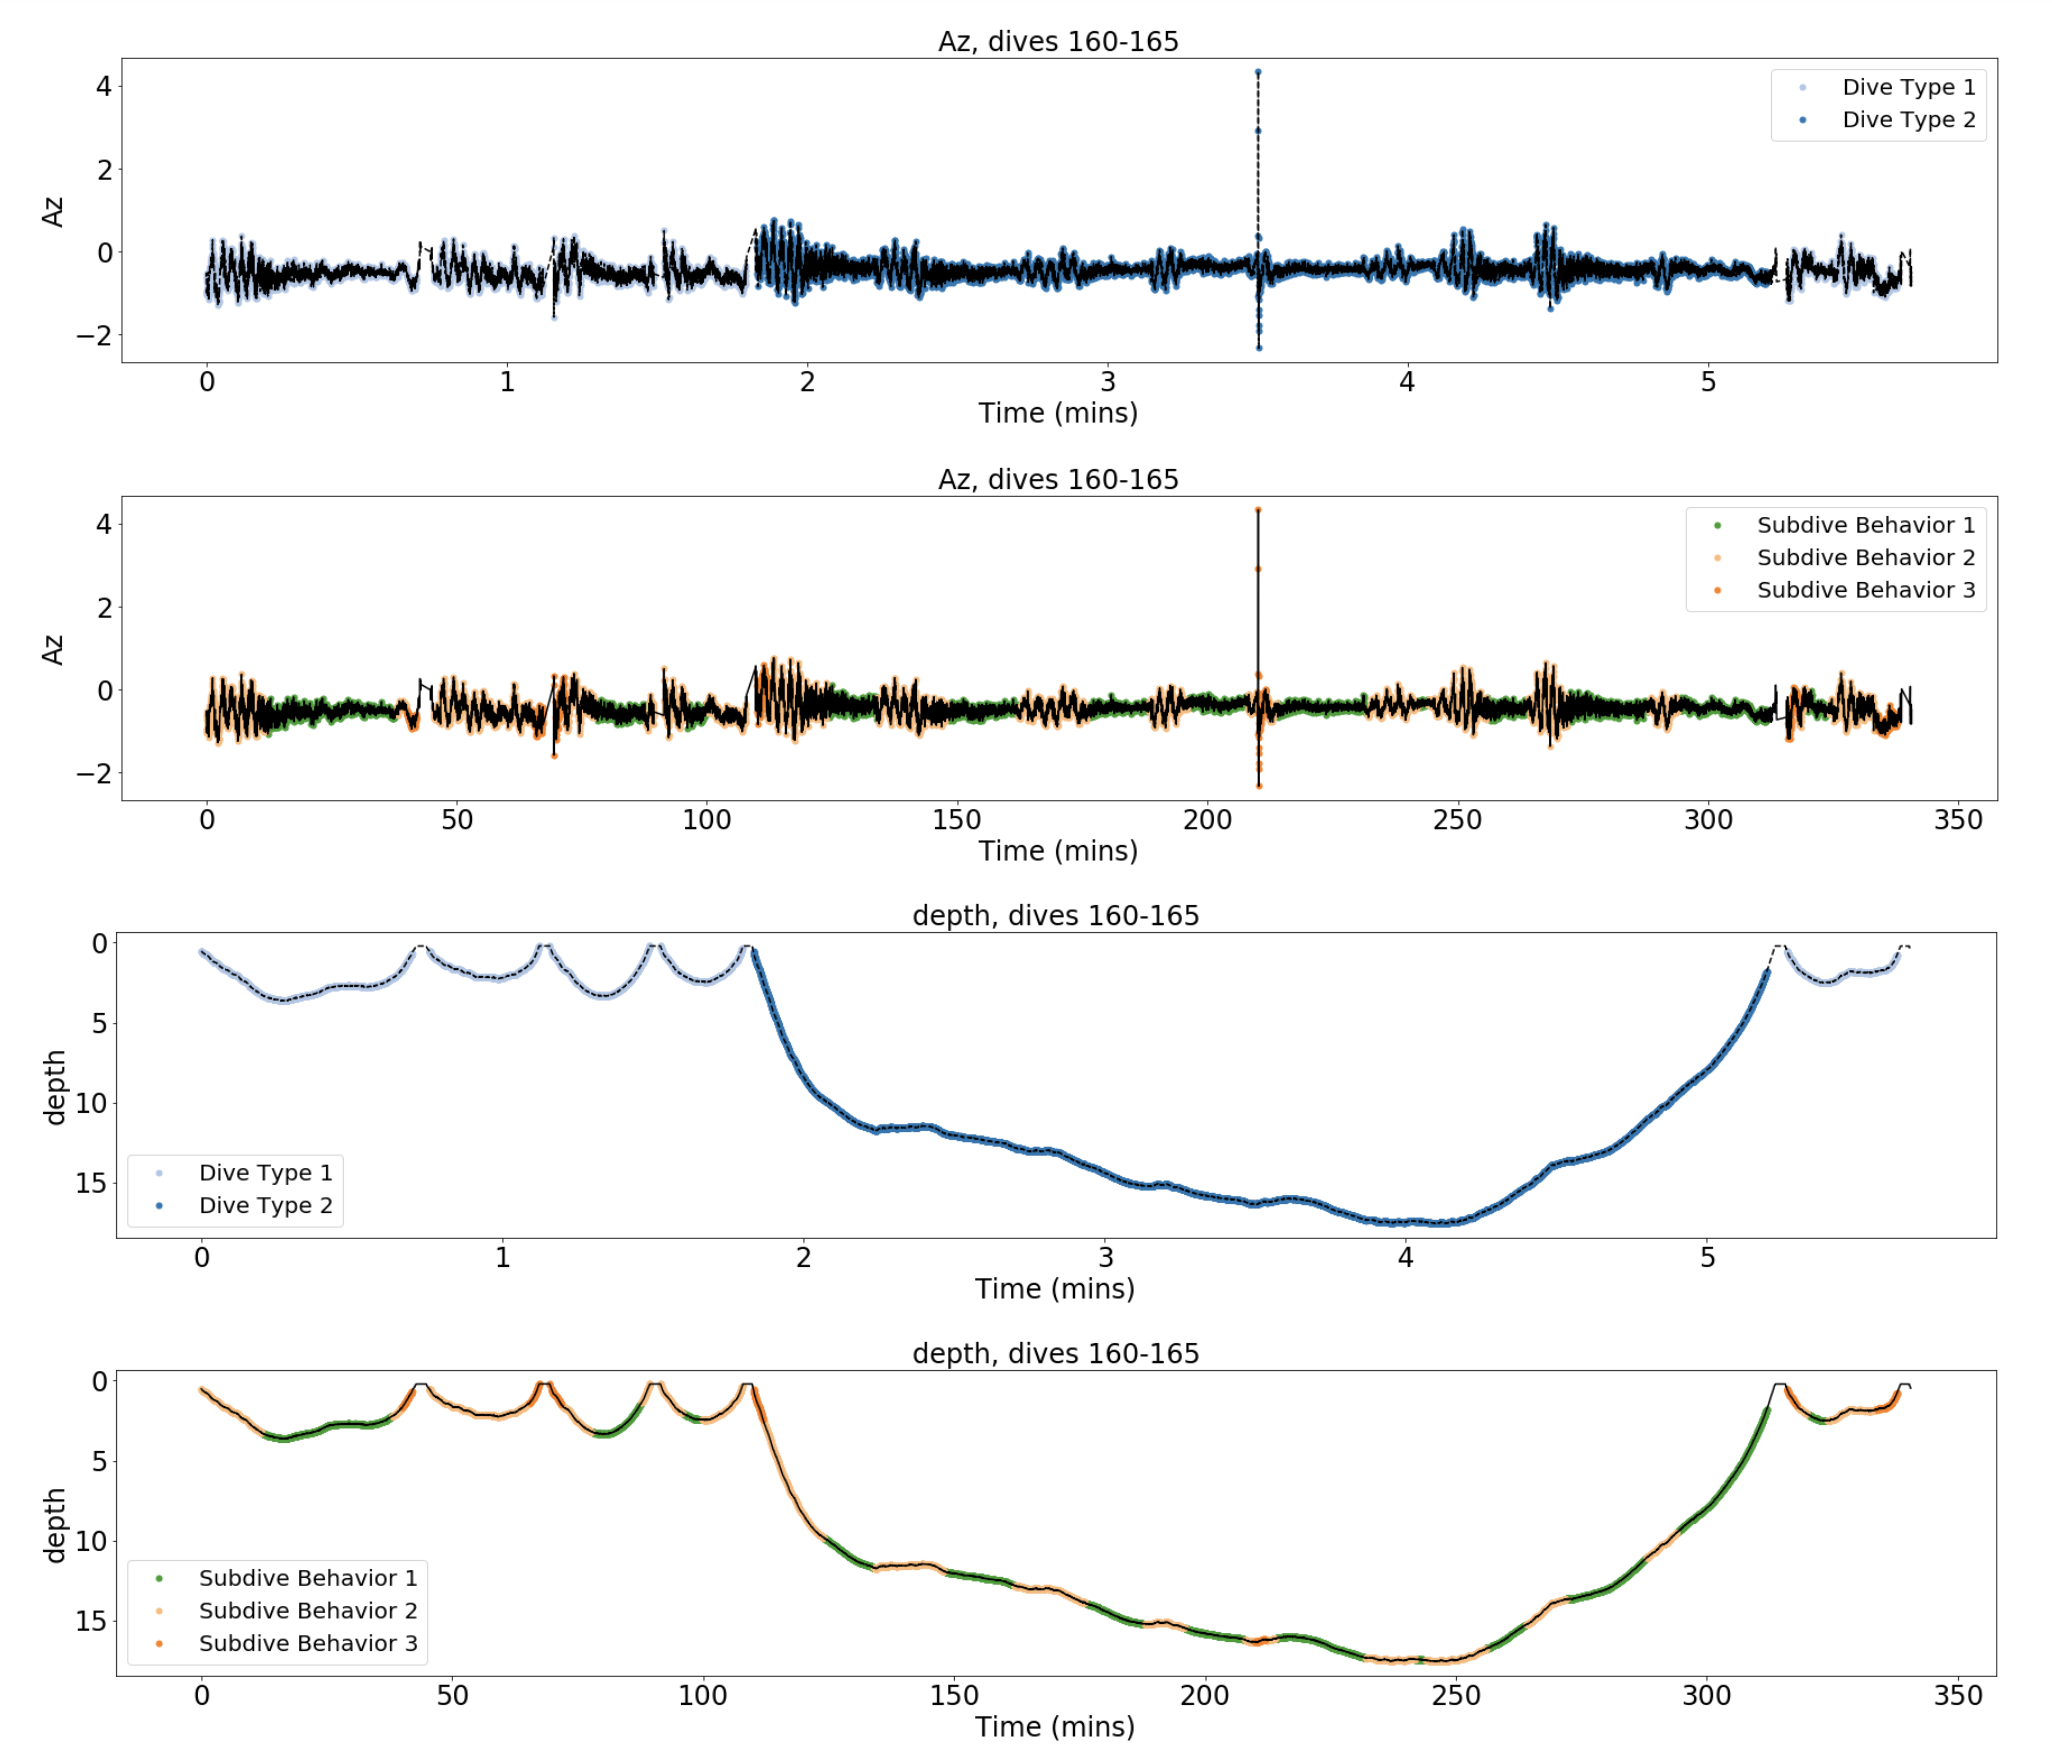
\includegraphics[width=5in]{../Plots/labeled_dives.png}
	\caption{Features of a particular set of killer whale dives and decoded estimates for the intra-dive behavioral states. The color of the plot corresponds to behavioral or dive state with the highest probability.}
	\label{fig:labeled_dives}
\end{figure}
%
\begin{figure}[ht]
	\centering
	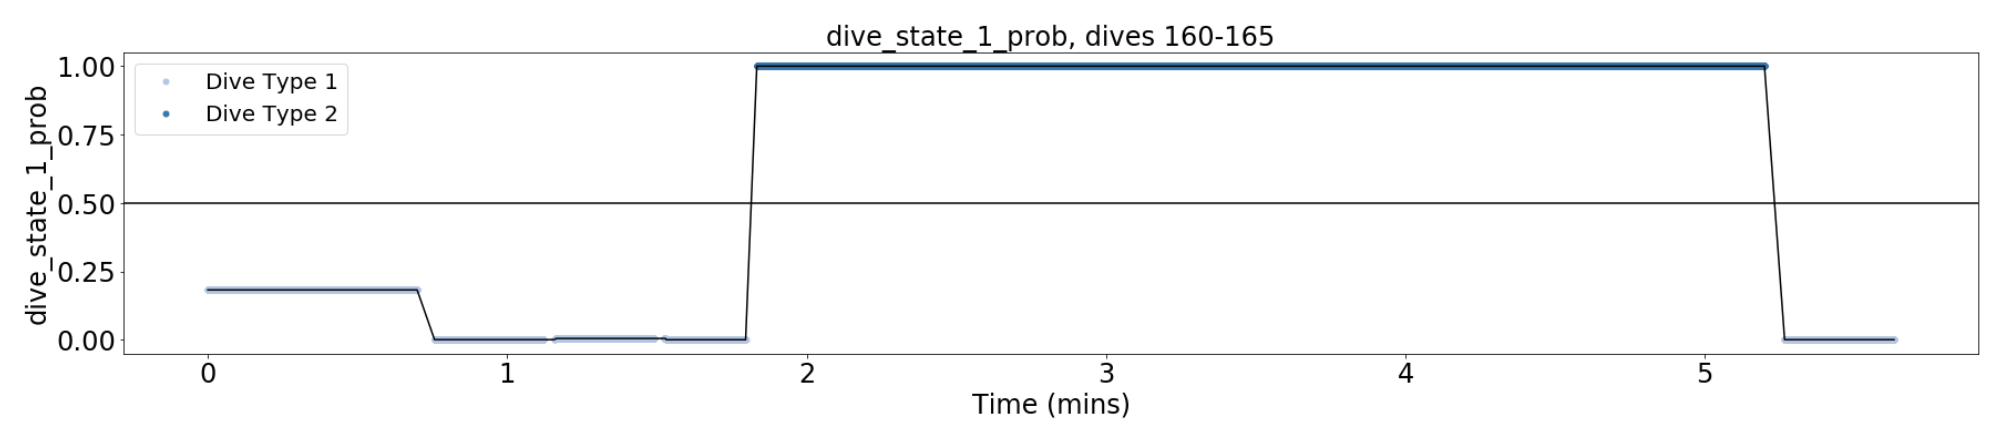
\includegraphics[width=5in]{../Plots/Coarse_state_probs.png}
	\caption{Probabilities of dive types for the set of killer whale dives from (fig \ref{fig:labeled_dives}).}
	\label{fig:coarse_probs}
\end{figure}
%
\begin{figure}[ht]
	\centering
	\begin{subfigure}[t]{1.0\textwidth}
        \centering
        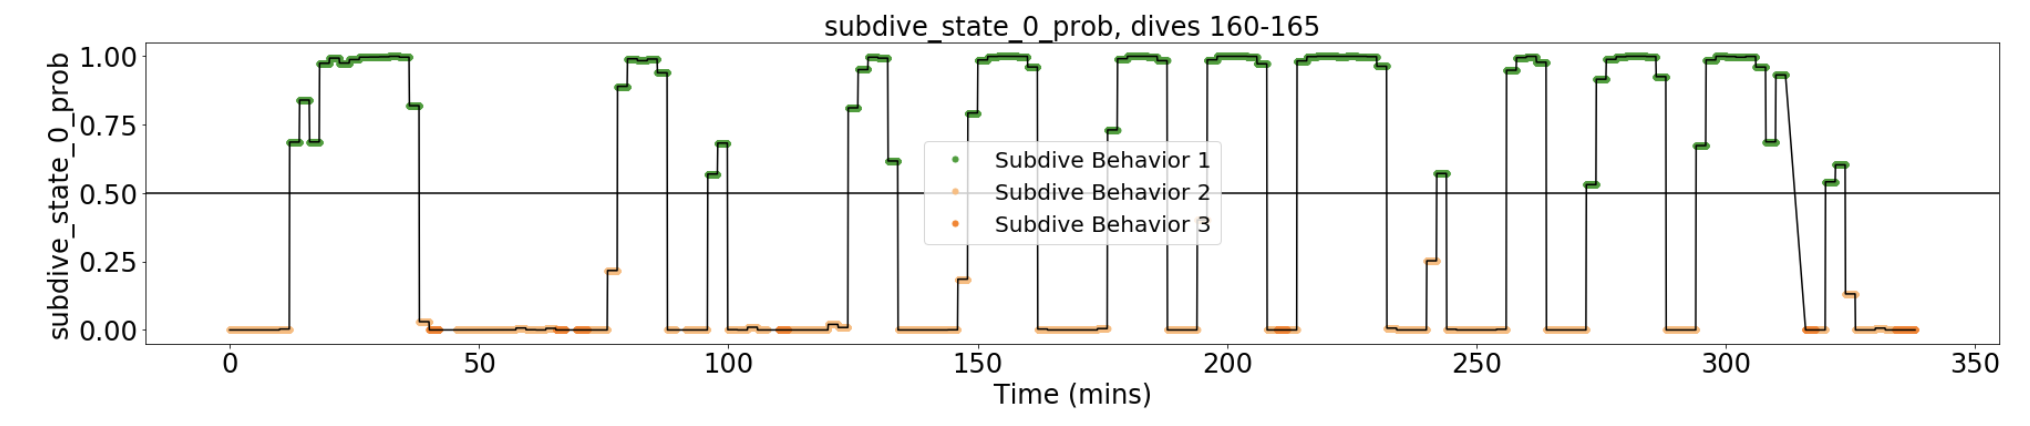
\includegraphics[width=5in]{../Plots/Fine_state_probs_1.png}
        \caption{Fine-scale state 1 probabilities}
    \end{subfigure}
    \newline
    \begin{subfigure}[t]{1.0\textwidth}
        \centering
        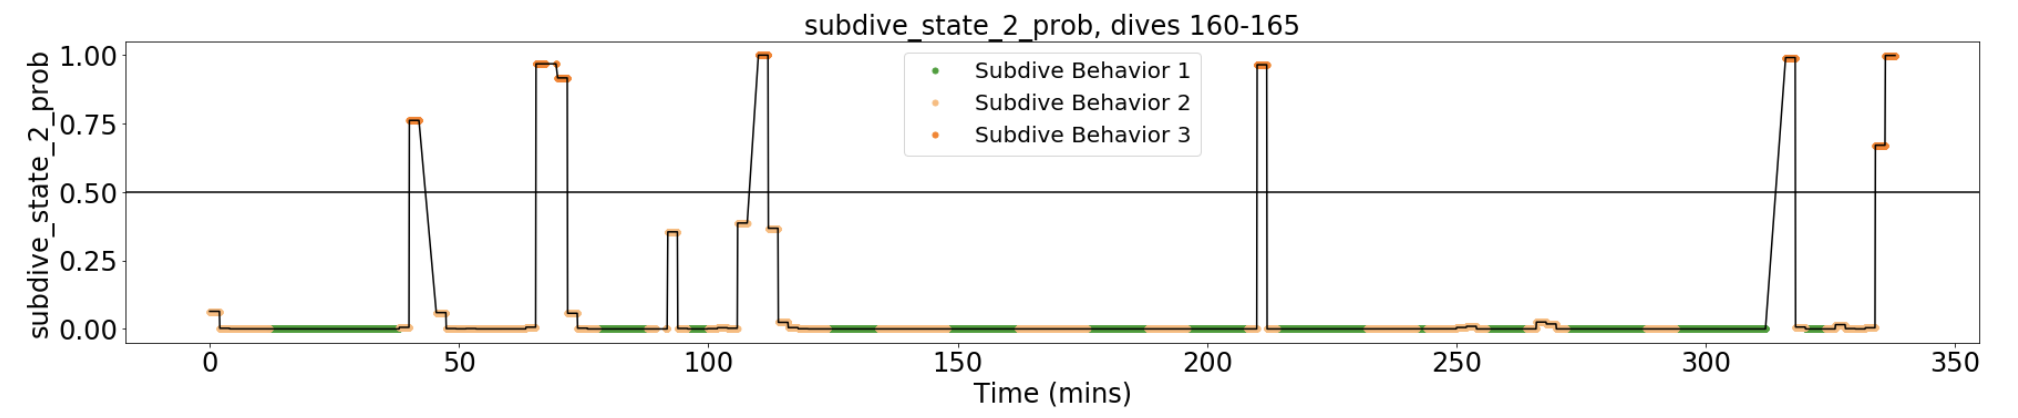
\includegraphics[width=5in]{../Plots/Fine_state_probs_3.png}
        \caption{Fine-scale state 3 probabilities}
    \end{subfigure}
	\caption{Probabilities of sub-dive types for the set of killer whale dives from (fig \ref{fig:labeled_dives}).}
	\label{fig:fine_probs}
\end{figure}

\subsection{Model Validation}
\label{subsec:model_validation}

Two visual tools were used to evaluate the model: pseudo-residuals and empirical histograms. A pseudo-residual of a particular observation is the marginal cdf of an observation, conditioned on all other observations, and mapped to the quantile function of a standard normal distribution (see \citep{Zucchini:2016} for details). In particular, the pseudo-residual of an observation $y_{t,s^*}$ is $\Phi^{-1} \left(Pr(Y_{t,s^*} < y_{t,s^*}|\{Y_1,\ldots,Y_T\}/\{Y_{t,s^*}\}) \right)$, where $\Phi$ is the cdf of a standard normal distribution. If the model is well-specified, then all pseudo-residuals should be independent and follow a standard normal distribution. While histograms of the pseudoresiduals support this for most observations, one notable exception is the case of $Y^{*(2)}$, shown in (fig \ref{fig:pseudoresids}), which are noticeably right-skewed. This implies that the true distribution of $Y^{*(2)}$ may follow a heavier-tailed distribution compared to a gamma distribution such as a power law. 

\begin{figure}[ht]
	\centering
	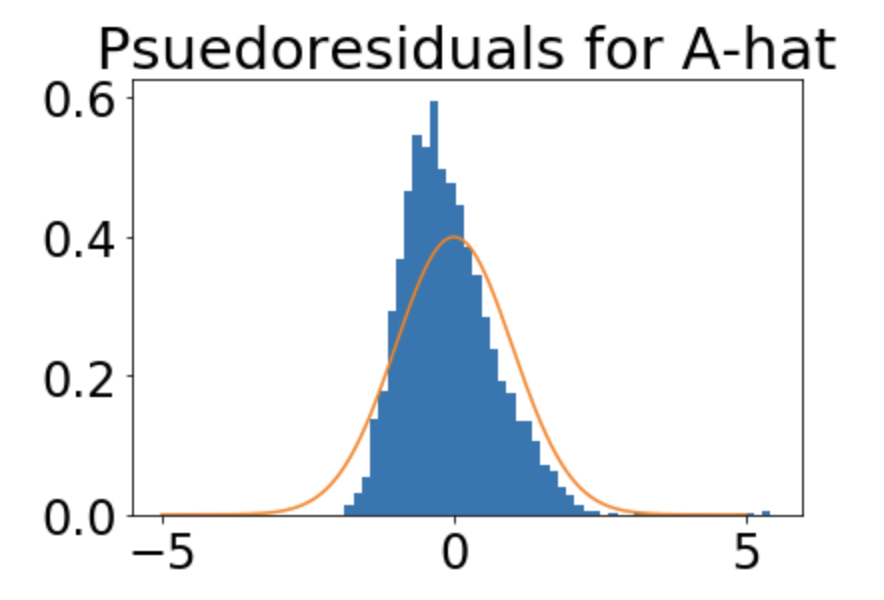
\includegraphics[width=5in]{../Plots/pseudoresids.png}
	\caption{Psuedoresiduals of $Y^{*(2)}$}
	\label{fig:pseudoresids}
\end{figure}

In addition to psuedoresiduals, we plotted histograms of observations for each feature within each hidden state. In particular, observations were weighted by the probability that the whale was in a particular hidden state. This empirical distribution was then plotted over the estimated true pdf of that feature for the hidden state. Again, our results mostly support the model in question with the exception of $Y^{*(2)}$, which is right-skewed. In addition, $Y^{*(1)}$ has heavy tails for sub-dive state 3 (see fig \ref{fig:empirical_dist}), indicating the existence of rare events corresponding to very violent trashing of the killer whale. These outliers are potential subjects for future studies to better understand rare behavioral events for this killer whale.

\begin{figure}[ht]
	\centering
	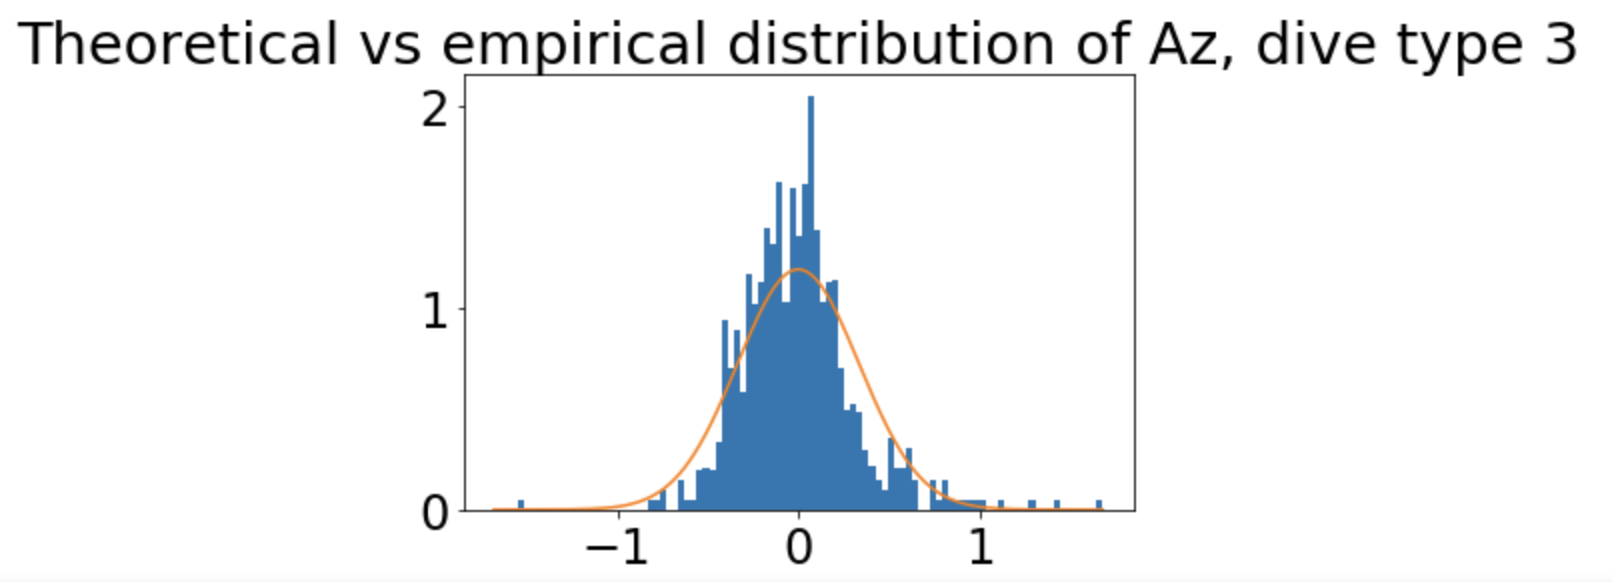
\includegraphics[width=5in]{../Plots/empirical_dist.png}
	\caption{Empirical distribution of $Y^{*(1)}_z$ for sub-dive state 3 plotted over its estimated pdf.}
	\label{fig:empirical_dist}
\end{figure}